\chapter{DEPLOYMENT}
\section{Folder Structure}

The project follows a standard MERN stack folder organization with clearly separated frontend and backend directories.

\begin{figure}[H]
    \centering
    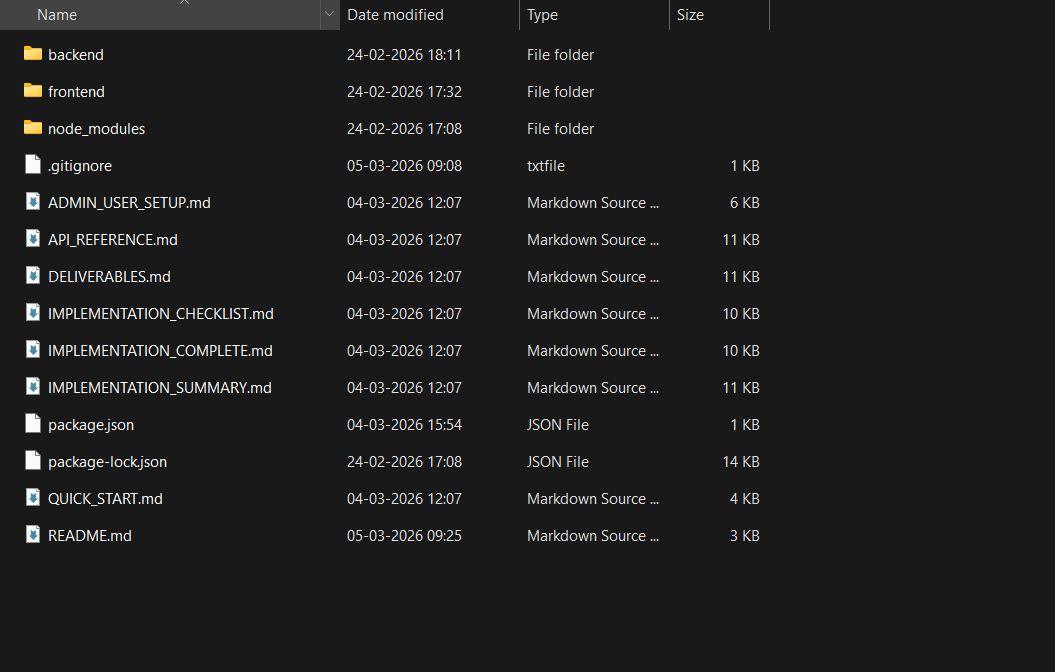
\includegraphics[width=0.75\textwidth]{image/folderr.png}
    \caption{Project Folder Structure}
    \label{fig:deployment_structure}
\end{figure}

\begin{figure}[H]
    \centering
    \begin{tikzpicture}[
        node distance=0.4cm,
        folder/.style={rectangle, draw=gray!60, fill=blue!5, rounded corners=2pt, minimum width=3.2cm, minimum height=0.55cm, font=\scriptsize\bfseries, align=left},
        file/.style={rectangle, draw=gray!40, fill=white, rounded corners=2pt, minimum width=3.2cm, minimum height=0.5cm, font=\scriptsize, align=left},
        conn/.style={draw=gray!50, thick}
    ]

    % Root
    \node[folder] (root) at (0,0) {sem4/};

    % Backend
    \node[folder, below right=0.5cm and -0.8cm of root] (backend) {backend/};
    \node[file, below=0.3cm of backend] (models) {models/};
    \node[file, below=0.3cm of models] (routes) {routes/};
    \node[file, below=0.3cm of routes] (config) {config/};
    \node[file, below=0.3cm of config] (middleware) {middleware/};
    \node[file, below=0.3cm of middleware] (serverjs) {server.js};

    % Frontend
    \node[folder, right=3cm of backend] (frontend) {frontend/};
    \node[file, below=0.3cm of frontend] (src) {src/};
    \node[file, below=0.3cm of src] (pages) {pages/};
    \node[file, below=0.3cm of pages] (components) {components/};
    \node[file, below=0.3cm of components] (context) {context/};
    \node[file, below=0.3cm of context] (utils) {utils/};

    % Connections
    \draw[conn] (root.south) -- ++(0,-0.2) -| (backend.north);
    \draw[conn] (root.south) -- ++(0,-0.2) -| (frontend.north);

    \foreach \child in {models, routes, config, middleware, serverjs}
        \draw[conn] (backend.south) ++(0.2,0) |- (\child.west);

    \foreach \child in {src, pages, components, context, utils}
        \draw[conn] (frontend.south) ++(0.2,0) |- (\child.west);

    \end{tikzpicture}
    \caption{Project Directory Tree Diagram}
    \label{fig:dir_tree}
\end{figure}

\section{Deployment Steps}

The application is deployed locally using the following steps:

\begin{enumerate}
    \item \textbf{Clone the Repository:} Pull the project from GitHub.
    \item \textbf{Install Dependencies:} Run \texttt{npm install} from the root directory, which installs both frontend and backend packages.
    \item \textbf{Configure Environment:} Set up the \texttt{.env} file in the backend folder with MongoDB Atlas connection string and JWT secret.
    \item \textbf{Start Backend Server:} Run \texttt{node server.js} from the backend directory. The server starts on port 5000.
    \item \textbf{Start Frontend Server:} Run \texttt{npm run dev} from the frontend directory. Vite serves the React application.
    \item \textbf{Seed Data:} On first startup, test users (admin and regular user) are auto-seeded. Product data can be seeded via the seed API endpoint.
\end{enumerate}